% Template inspired by Drew Ulick
% https://www.overleaf.com/articles/130-cheat-sheet/ntwtkmpxmgrp
\documentclass{article}
\usepackage[landscape]{geometry}
\usepackage{xifthen}
\usepackage{url}
\usepackage{hyperref}
\usepackage{xcolor}
\hypersetup{
    colorlinks=true,
    linkcolor=black
}
\usepackage{tikz}
\usetikzlibrary{positioning,fit,calc,backgrounds}

\usepackage{xcolor}
\usepackage{enumitem}
\usepackage{amssymb, amsmath,endnotes}
\usepackage{multicol}
\usepackage{multirow}
\usepackage{fontawesome}
\usepackage{xparse}
\usepackage{listings}
\usepackage[utf8]{inputenc}
\usepackage[listings]{tcolorbox}
\tcbuselibrary{listings}
\lstdefinestyle{simple}{ %
    basicstyle=\ttfamily,
    breaklines = true,
    backgroundcolor=\color{gray!30},
}
\lstdefinestyle{bash}{ %
  backgroundcolor=\color{gray!30},   % choose the background color; you must add \usepackage{color} or \usepackage{xcolor}; should come as last argument
  basicstyle=\ttfamily\footnotesize\color{black},        % the size of the fonts that are used for the code
  breakatwhitespace=false,         % sets if automatic breaks should only happen at whitespace
  breaklines=true,                 % sets automatic line breaking
  escapeinside={\%*}{*)},          % if you want to add LaTeX within your code
  extendedchars=true,              % lets you use non-ASCII characters; for 8-bits encodings only, does not work with UTF-8
  frame=single	                   % adds a frame around the code
  keepspaces=true,                 % keeps spaces in text, useful for keeping indentation of code (possibly needs columns=flexible)
  language=bash,                 % the language of the code
  keywordstyle=\bfseries,
  morekeywords={GET,POST,PUT,DELETE,... },           % if you want to add more keywords to the set
  numbers=left,                    % where to put the line-numbers; possible values are (none, left, right)
  numbersep=5pt,                   % how far the line-numbers are from the code
  numberstyle=\tiny\color{black}, % the style that is used for the line-numbers
  rulecolor=\color{black},         % if not set, the frame-color may be changed on line-breaks within not-black text (e.g. comments (green here))
  showspaces=false,                % show spaces everywhere adding particular underscores; it overrides 'showstringspaces'
  showstringspaces=false,          % underline spaces within strings only
  showtabs=false,                  % show tabs within strings adding particular underscores
  stepnumber=1,                    % the step between two line-numbers. If it's 1, each line will be numbered
  tabsize=2,	                   % sets default tabsize to 2 spaces
}
\lstdefinelanguage{json}{
    keywords={GET,POST,PUT,DELETE},
    keywordstyle=\color{darkgray!70!black}\bfseries,
    identifierstyle=\color{black},
    sensitive=false,
    comment=[l]{//},
    morecomment=[s]{/*}{*/},
    commentstyle=\color{purple}\ttfamily,
    stringstyle=\color{green!50!black}\ttfamily,
    morestring=[b]',
    morestring=[b]"
}
\lstdefinestyle{js}{ %
  backgroundcolor=\color{gray!30},   % choose the background color; you must add \usepackage{color} or \usepackage{xcolor}; should come as last argument
  basicstyle=\ttfamily\footnotesize\color{black},        % the size of the fonts that are used for the code
  breakatwhitespace=false,         % sets if automatic breaks should only happen at whitespace
  breaklines=true,                 % sets automatic line breaking
  escapeinside={\%*}{*)},          % if you want to add LaTeX within your code
  extendedchars=true,              % lets you use non-ASCII characters; for 8-bits encodings only, does not work with UTF-8
  frame=single	                   % adds a frame around the code
  keepspaces=true,                 % keeps spaces in text, useful for keeping indentation of code (possibly needs columns=flexible)
  language=json,                 % the language of the code
%   keywordstyle=\bfseries,
%   morekeywords={GET,POST,PUT,DELETE,... },           % if you want to add more keywords to the set
  numbers=none,                    % where to put the line-numbers; possible values are (none, left, right)
  numbersep=5pt,                   % how far the line-numbers are from the code
  numberstyle=\tiny\color{black}, % the style that is used for the line-numbers
  rulecolor=\color{black},         % if not set, the frame-color may be changed on line-breaks within not-black text (e.g. comments (green here))
  showspaces=false,                % show spaces everywhere adding particular underscores; it overrides 'showstringspaces'
  showstringspaces=false,          % underline spaces within strings only
  showtabs=false,                  % show tabs within strings adding particular underscores
  stepnumber=1,                    % the step between two line-numbers. If it's 1, each line will be numbered
  tabsize=2,	                   % sets default tabsize to 2 spaces
}
\lstset{style=simple}

\title{MISP Cheat Sheet (FR)}
\author{MISP Project}
\date{\today}

\makeatletter
\newcommand{\linkdest}[1]{\Hy@raisedlink{\hypertarget{#1}{}}}
\let\theauthor\@author
\let\thedate\@date
\makeatother
\advance\topmargin-.8in
\advance\textheight3in
\advance\textwidth3in
\advance\oddsidemargin-1.5in
\advance\evensidemargin-1.5in
\parindent0pt
\parskip2pt

%
% MISP ELEMENTS
%
\newcommand{\hr}{\centerline{\rule{3.5in}{1pt}}}
\newcommand{\misp}{
\includegraphics[scale=0.2]{misp.pdf}\hspace*{0.5em}}
\newcommand{\events}{\hyperlink{event}{\texttt{Events}} }
\newcommand{\event}{\hyperlink{event}{\texttt{Event}} }
\newcommand{\attributes}{\hyperlink{attribute}{\texttt{Attributes}} }
\newcommand{\attribute}{\hyperlink{attribute}{\texttt{Attribute}} }
\newcommand{\objects}{\hyperlink{object}{\texttt{MISP Objects}} }
\newcommand{\object}{\hyperlink{object}{\texttt{MISP Object}} }
\newcommand{\reference}{\hyperlink{reference}{\texttt{Reference}} }
\newcommand{\references}{\hyperlink{reference}{\texttt{References}} }
\newcommand{\proposals}{\hyperlink{proposal}{\texttt{Proposals}} }
\newcommand{\proposal}{\hyperlink{proposal}{\texttt{Proposal}} }
\newcommand{\eventreports}{\hyperlink{eventreport}{\texttt{Event Reports}} }
\newcommand{\eventreport}{\hyperlink{eventreport}{\texttt{Event Report}} }
\newcommand{\sightings}{\hyperlink{sighting}{\texttt{Sightings}} }
\newcommand{\sighting}{\hyperlink{sighting}{\texttt{Sighting}} }
\newcommand{\taxonomies}{\texttt{Taxonomies }}
\newcommand{\taxonomy}{\texttt{Taxonomy }}
\newcommand{\galaxy}{\hyperlink{galaxy}{\texttt{Galaxy}} }
\newcommand{\galaxies}{\hyperlink{galaxy}{\texttt{Galaxies}} }
\newcommand{\clusters}{\hyperlink{cluster}{\texttt{Galaxy Clusters}} }
\newcommand{\cluster}{\hyperlink{cluster}{\texttt{Galaxy Cluster}} }
\newcommand{\sharinggroups}{\hyperlink{sharinggroup}{\texttt{Sharing Groups}} }
\newcommand{\sharinggroup}{\hyperlink{sharinggroup}{\texttt{Sharing Group}} }
\newcommand{\notes}{\hyperlink{note}{\texttt{Analyst Notes}} }
\newcommand{\note}{\hyperlink{note}{\texttt{Analyst Note}} }
\newcommand{\opinions}{\hyperlink{opinion}{\texttt{Analyst Opinions}} }
\newcommand{\opinion}{\hyperlink{opinion}{\texttt{Analyst Opinion}} }
\newcommand{\relationships}{\hyperlink{relationship}{\texttt{Analyst Relationships}} }
\newcommand{\relationship}{\hyperlink{relationship}{\texttt{Analyst Relationship}} }
\newcommand{\collections}{\hyperlink{collection}{\texttt{Element Collections}} }
\newcommand{\collection}{\hyperlink{collection}{\texttt{Element Collection}} }

\newcommand{\taggable}{\faicon{tags}\hspace*{0.3em}}
\newcommand{\distributable}{\faicon{eye-slash}\hspace*{0.3em}}
\newcommand{\synchronisable}{\faicon{exchange}\hspace*{0.3em}}

%
% Layout
%
\tikzstyle{mybox} = [
    draw=black,
    fill=white,
    very thick,
    rectangle, rounded corners,
    inner sep=10pt
]
\tikzstyle{boxtitle} = [
    % fill=black,
    % text=white,
    % fill=gray!30,
    % text=black,
    % font=\bfseries,
    % right=10pt
    draw=black,
    line width=1pt,
    text=white,
    fill=black!80,
    font=\bfseries,
    rectangle, rounded corners=2pt,
    inner sep=4pt,
    right=10pt
]
\tikzset{actionbox/.style={
    text=white,
    yshift=-1pt,xshift=-1pt,
    append after command={
    \pgfextra
            \draw[sharp corners, fill=black]% 
        (\tikzlastnode.west)% 
        [rounded corners=0pt] |- (\tikzlastnode.north)% 
        [rounded corners] -| (\tikzlastnode.east)% 
        [rounded corners=0pt] |- (\tikzlastnode.south)% 
        [rounded corners] -| (\tikzlastnode.west);
    \endpgfextra
    }
}}

% Creates a box with a label taking 1/3 of the available width
% arg1[optional] = icon
% arg2[optional] = purpose
% arg3[optional] = usecase
% arg4[optional] = actions
% arg5[optional] = description
% arg6 = title
% arg7 = content
\NewDocumentCommand{\cheatbox}{ O{} O{} O{} O{} O{} m m}{
    \begin{tikzpicture}
        \node [mybox] (box){%
            \begin{minipage}{0.3\textwidth}
            \ifthenelse{\isempty{#4}}{}{\vspace{1em}}
            \textit{#5}
            \vspace*{0.3em}
            \ifthenelse{\isempty{#2}}{}{ \par{\textbf{Purpose}: #2}}
            \ifthenelse{\isempty{#3}}{}{ \par{\textbf{Usecase}: #3\ifthenelse{\isempty{#7}}{}{\\}}}
            #7
            \end{minipage}
        };
        \node[boxtitle] at (box.north west) {#1 #6};
        \ifthenelse{\isempty{#4}}{}{
            \path node [actionbox, anchor=north east] at (box.north east) (actionLabel) {#4};
        }
    \end{tikzpicture}

    \vspace*{2pt}
}

% Creates a box with a label taking 0.46 of the available width
% arg1[optiona] = description
% arg2 = title
% arg3 = content
\newcommand{\cheatboxlarge}[3][]{
    \begin{tikzpicture}
        \node [mybox] (box){%
            \begin{minipage}{0.46\textwidth}
            \ifthenelse{\isempty{#1}}{}{\textit{#1}}
            \ifthenelse{\isempty{#1}}{}{\vspace{2pt}}
            #3
            \end{minipage}
        };
        \node[boxtitle] at (box.north west) {#2};
    \end{tikzpicture}

    \vspace*{3pt}
}

% Creates a formated entry in a \cheatbox
% arg1 = label
% arg2 = text
\newcommand{\boxentry}[2]{
    \par{\textbf{#1}: #2\vspace*{0.3em}}
}

% Creates a formated entry in a \cheatbox without additional spacing
% arg1 = label
% arg2 = text
\newcommand{\boxentrycompact}[2]{
    \par{\textbf{#1} #2}
}

% Creates a centered text for the available width with color formating
% arg1[optional, default=black] = bg color
% arg2[optional, default=white] = text color
% arg3 = text
\NewDocumentCommand{\multicolstitle}{O{black} O{white} m}{
    \begin{minipage}{0.46\textwidth}
        \begin{center}
            \colorbox{#1}{\Large\textcolor{#2}{\textbf{#3}}}
        \end{center}
    \end{minipage}
}

\newcommand{\bashcode}[1]{
    \colorbox{gray!20}{\lstinline[language=bash]|#1|}
}
\newcommand{\clicode}[1]{
    \colorbox{gray!20}{\lstinline[language=bash]|MISP/app/Console/cake #1|}
}
\newcommand{\httpcode}[3][]{\colorbox{gray!20}{#2 \lstinline[]|#3|}
    \colorbox{gray!20}{\lstinline[]|#1|}
}

\begin{document}
    \begin{center}{
    \huge{\textbf{MISP Concepts Cheat sheet (FR)}}}\\
\end{center}

\begin{multicols*}{2}
\cheatboxlarge{Glossary}{
    \boxentry{Correlations}{Relations créées automatiquement depuis un \attribute. Elles permettent l'inter-connexion entre \events basés sur leurs \attributes.}
    \boxentry{Correlation engine}{Système utilisé par MISP pour créer des correlations entre la valeur des \attribute. Il supporte actuellement la comparaison stricte de chaines de caractères, SSDEEP et les blocks CDIR.}
    \boxentry{Caching}{Processus de récupération de données d'une instance ou d'un feed afin de sauver les hashs des valeurs récupérées servant à la corrélation et la recherche.}    
    \boxentry{Delegation}{Acte de transférer la propriété d'un event vers une autre organisation tout en cachant le créateur original afin de garantir l'anonymat}    
    \boxentry{Deletion (hard/soft)}{\textit{Hard deletion} est l'acte de supprimer un element du système; Cela ne va pas révoquer la donnée sur les autres systèmes contrairement à la \textit{Soft deletion} où la révocation est propagée sur le réseau d'instances connectées.}
    \boxentry{Extended Event}{\event qui en étend un autre, permetant d'avoir une vue combinée. L'organisation qui a étendu l'\event est le propriétaire de l'extension . Cela permet à n'importe qui d'étendre n'importe quel \events et d'en avoir le contrôle.}
    \boxentry{\galaxy Matrix}{Matrice dérivée d'un \clusters appartenant à la même \galaxy. La structure (pages et colones) est définie au niveau de la \galaxy et son contenu provient des méta-données des \clusters.}
    \boxentry{Indicators}{\attribute contenant un pattern utile pour détecter une activité suspicieuse ou malveillante. Ils ont souvent la propriété \texttt{to\_ids} activée.}
    \boxentry{Orgc / Org}{\textit{L'organisation créatrice} (\textbf{Orgc}) est l'organisation qui a créé les données et qui est la seule à pouvoir les modifier. \textit{L'organisation propriétaire} (\textbf{Org}) est l'organisation qui possède les données et qui peut consulter le contenu. \textbf{Orgc} \& \textbf{Org} ne sont pas nécessairement les mêmes organisations.}
    \boxentry{Publishing}{Action de déclarer qu'un \event peut être synchronisé. Ce processus peut aussi envoyer des notifications et permet certains types de format d'export.}
    \boxentry{Pulling}{Action d'utiliser un utilisateur depuis une autre instance pour récupérer les données accessibles et les stoquer localement.}
    \boxentry{Pushing}{Action d'utiliser une connexion via un \textit{sync. user} pour envoyer des données à une autre instance.}
    \boxentry{Synchronisation}{Est l'échange de données entre deux (ou plus) instances MISP par le mécanisme de \textit{pull} ou \textit{push}.}
    \boxentry{Sync. filtering rule}{Peuvent être appliquées sur un lien de synchronisation pour le \textit{pull} ou \textit{push} afin de bloquer ou pemettre à des données d'être transférées.}
    \boxentry{Sync. User}{Rôle spécial pour un utilisateur donnant des permissions de synchronisation supplémentaires. L'utilisation des \textit{sync users} est la manière recommandée de configurer la synchronisation via \textit{push}.}
    \boxentry{Proposals}{Mécanisme pour proposer des modifications à l'organisation créatrice (\textbf{Orgc}). Si un chemin entre les instances existe, le \proposal pourra être synchronisé permetant au créateur de l'accepter ou de le refuser.}
}

\columnbreak
% arg1 = current distri level
% arg2 = text
\newcommand{\changestyledistribution}[2]{
    \ifthenelse{#1 > #2}{
        \tikzset{currentstyle/.style=fullnode}
    }{
        \tikzset{currentstyle/.style=emptynode}
    }
}
% arg1 = current distri level
\newcommand{\distrigraph}[1]{
    \def \scale {0.2}
    \def \scaletext {0.1}
    \begin{tikzpicture}[
        emptynode/.style={circle, draw=black, scale=\scale},
        fullnode/.style={circle, draw=black, fill=black, scale=\scale},
        textnode/.style={scale=0.7, inner sep=3pt,xshift=-2pt},
    ]
    \tikzset{
        currentstyle/.style={}
    }
        \changestyledistribution{#1}{0}
        \node[currentstyle] (d0)  {};
        \changestyledistribution{#1}{1}
        \node[currentstyle] (d1a) [above right= 1pt and 30pt of d0] {};
        \node[currentstyle] (d1b) [below right= 1pt and 30pt of d0] {};
        \changestyledistribution{#1}{2}
        \node[currentstyle]  (d2)  [right=of d1b] {};
        \changestyledistribution{#1}{2}
        \node[currentstyle]  (d3)  [right=of d2] {};

        \node[textnode] (d0-notice) [above= 10pt of d0] {$n=0$};
        \node[textnode] (d1a-notice) [above= 5pt of d1a] {$n=1$};
        \node[textnode] (d2-notice) [above= 15pt of d2] {$n=2$};
        \node[textnode] (d3-notice) [above= 15pt of d3] {$n=3$};

        \draw[-] (d0) to[out=30, in=180] (d1a);
        \draw[-] (d0) to[out=-30, in=180] (d1b);
        \draw[-] (d1b) -- (d2);
        \draw[-] (d2) -- (d3);

        % \draw[-] (d0-notice.east) -- +(15pt,0pt) -- (d0.135);
        % \draw[-] ($(d0-notice.east) + (-1pt,-2pt)$) -- ($(d0) + (-3pt,2pt)$);
    \end{tikzpicture}
}

\newcommand{\createdistrilegend}{
    \def \scale {0.2}
    \begin{tikzpicture}[
        emptynode/.style={circle, draw=black, scale=\scale},
        fullnode/.style={circle, draw=black, fill=black, scale=\scale},
        textnode/.style={scale=0.7, inner sep=3pt,xshift=-2pt},
    ]
        \node[emptynode] (empty) {};
        \node[fullnode] (full) [below=5pt of empty] {};
        \node[textnode] () [right=3pt of empty] {Does not have the Event};
        \node[textnode] () [right=3pt of full] {Has the Event};
    \end{tikzpicture}
}
\cheatboxlarge[Contrôle qui peut voir les données et comment elles doivent être synchronisées.]{Distribution}{
    \boxentry{Organisation only}{Seulement les membres de l'organisation}
    \boxentry{This community}{Les organisations sur l'instance MISP}
    \boxentry{Connected Communities}{Les organisations sur l'instance et celles d'autres instances se synchronisant dessus. Lorsque les données sont reçues, leur distribution est réduite à \texttt{This community} afin d'éviter d'autres propagations. ($n\leq 1$)}
    \vspace*{-0.7em}
    \begin{center}
        \createdistrilegend
        \hspace*{1em}
        \distrigraph{2}
    \end{center}
    \boxentry{All Communities}{Tous ceux ayant accès. Les données seront propagées librement dans le réseau d'instances connectées. ($n = \infty$)}
    \vspace*{-0.7em}
    \begin{center}\distrigraph{3}\end{center}
    \boxentry{\linkdest{sharinggroup}Sharing Groups}{Liste de distribution qui énumère la liste des organisations ayant accès aux données et comment celles-ci doivent être synchronisées.}

    \begin{multicols*}{2}
        \begin{center}
            \begin{tabular}{| l | l |}
                \hline
                \multicolumn{2}{|c|}{\sharinggroup configuration} \\
                \hline
                \multirow{3}{*}{Organisations} & Org. $\alpha$\\
                    & Org. $\omega$\\
                    & Org. $\gamma$\\
                \hline
                \multirow{3}{*}{Instances*} & MISP 1\\
                    & MISP 2\\
                    & MISP 3\\
                \hline
            \end{tabular}\\
            *Ou activé le mode roaming à la place
        \end{center}
        \columnbreak

        \begin{center}
            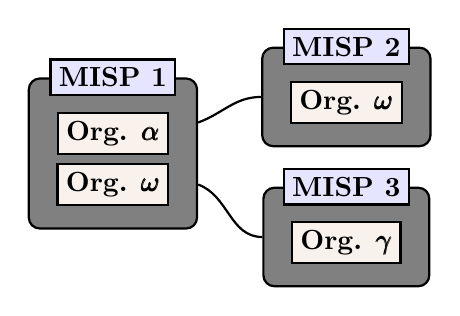
\begin{tikzpicture}[
    node/.style={inner sep=0pt},
    simplebox/.style n args={3}{
        rectangle, rounded corners, thick,
        draw=black, fill=#1,
        minimum width=#2,
        minimum height=#3,
        inner sep=10pt, inner ysep=10pt
    },
    simpleboxtitle/.style = {
        rectangle, rounded corners=0,
        minimum width=1em,
        fill=brown!10, text=black, draw, thick,
        font=\bfseries,
        inner sep=3pt
    },
    header/.style = {%
        inner ysep = +1.0em,
        append after command = {
            \pgfextra{\let\TikZlastnode\tikzlastnode}
            node[simpleboxtitle] (header-\TikZlastnode) at (\TikZlastnode.north) {#1}
        }
    },
    coloredHeader/.style n args={2}{
        inner ysep = +1.0em,
        append after command = {
            \pgfextra{\let\TikZlastnode\tikzlastnode}
            node[simpleboxtitle,fill=#2] (header-\TikZlastnode) at (\TikZlastnode.north) {#1}
        }
    }
]

    \node[simpleboxtitle] (orgs01) [] {Org. $\pmb{\alpha}$};
    \node[simpleboxtitle] (orgs02) [below = 0.3em of orgs01] {Org. $\pmb{\omega}$};
    \node[fit = (orgs01) (orgs02)] (orgs0) {};
    \node[simpleboxtitle] (orgs1) [above right= -0.8em and 4em of orgs0] {Org. $\pmb{\omega}$};
    \node[simpleboxtitle] (orgs2) [below = 3.5em of orgs1] {Org. $\pmb{\gamma}$};
    \begin{scope}[on background layer]
        \node[yshift=2pt, fit = (orgs01) (orgs02), simplebox={gray}{1em}{2em}, coloredHeader={MISP 1}{blue!10}] (m1) {};
        \node[yshift=2pt, fit = (orgs1), simplebox={gray}{1em}{2em}, coloredHeader={MISP 2}{blue!10}] (m2) {};
        \node[yshift=2pt, fit = (orgs2), simplebox={gray}{1em}{2em},  coloredHeader={MISP 3}{blue!10}] (m3) {};
    \end{scope}

    \draw[-, thick] (m1) to[out=20, in=180] (m2);
    \draw[-, thick] (m1) to[out=-20, in=180] (m3);
\end{tikzpicture}
        \end{center}
    \end{multicols*}
}

\cheatboxlarge[L'acte de partager où tout le monde peut être un consommateur et/ou un producteur.]{Synchronisation}{
    Une synchronisation dans un sens entre deux instances MISP. L'organisation $\alpha$ avait créé un \textit{sync user} \faicon{user-plus} sur MISP 2 et a noté la clé API générée. Un lien de synchronisation peut être créé sur MISP 1 en utilisant cette clé API et l'organisation du \textit{sync user}. Dès lors, MISP 1 peut \textit{pull} des données depuis MISP 2 et \textit{push} des données vers MISP 2.
    \begin{center}
        \pgfdeclarelayer{bg0}    % declare background layer
\pgfdeclarelayer{bg1}    % declare background layer
\pgfsetlayers{bg0,bg1,main}  % set the order of the layers (main is the standard layer)
\begin{tikzpicture}[
    simplebox/.style n args={3}{
        rectangle, rounded corners, thick,
        draw=black, fill=#1,
        minimum width=#2,
        minimum height=#3,
        inner sep=10pt, inner ysep=10pt
    },
    simpleboxtitle/.style = {
        rectangle, rounded corners=0,
        minimum width=1em,
        fill=brown!10, text=black, draw, thick,
        font=\bfseries,
        inner sep=3pt
    },
    header/.style = {%
        inner ysep = +1.0em,
        append after command = {
            \pgfextra{\let\TikZlastnode\tikzlastnode}
            node[simpleboxtitle] (header-\TikZlastnode) at (\TikZlastnode.north) {#1}
        }
    },
    coloredHeader/.style n args={2}{
        inner ysep = +1.0em,
        append after command = {
            \pgfextra{\let\TikZlastnode\tikzlastnode}
            node[simpleboxtitle,fill=#2] (header-\TikZlastnode) at (\TikZlastnode.north) {#1}
        }
    },
    user/.style = {
        inner sep=0pt
    },
    legend/.style = {
        rectangle, rounded corners=0,
        inner sep=2pt,
        draw=black
    },
    nodes = {align = center}
]

    \node[user] (misp1users) {\faicon{user} \faicon{user} \faicon{user}};
    \node[user] (misp2users) [right= 13em of misp1users] {\faicon{user} \faicon{user}};
    \node[user] (misp2users2) [right= 3em of misp2users] {\faicon{user} \faicon{user} \faicon{user}};
    \node[user,inner xsep=3pt] (syncuser) [left= 0.0em of misp2users] {\faicon{user-plus}};
    \begin{pgfonlayer}{bg1}
        \node[yshift=2pt, fit = (misp1users), simplebox={white}{1em}{2em}, header = Org. $\pmb{\alpha}$] (misp1org) {};
        \node[yshift=2pt, fit = (misp2users) (syncuser), simplebox={white}{1em}{2em}, header = Org. $\pmb{\alpha}$] (misp2org) {};
        \node[yshift=2pt, fit = (misp2users2), simplebox={gray!30}{1em}{2em}, header = Org. $\pmb{\omega}$] (misp2org2) {};
    \end{pgfonlayer}
    \begin{pgfonlayer}{bg0}
        \node[yshift=+0.5em, fit = (misp1org), simplebox={gray}{11em}{6em}, coloredHeader={MISP 1}{blue!10}] (m1) {};
        \node[yshift=+0.5em, fit = (misp2org) (misp2org2), simplebox={gray}{11em}{6em}, coloredHeader={MISP 2}{blue!10}] (m2) {};
    \end{pgfonlayer}
    \draw[-,very thick] (m1.south) -- ++(0,-15pt) -| ($(syncuser.south) + (0,-2pt)$) node [
        pos=0.25,above,yshift=-0.9em
    ] (textsync) {Sync. connection};
    \def \offsetY {3}
    \draw[->,thick] ($(m1.east) + (1pt,\offsetY pt)$) -- ($(m2.west) + (-1pt,\offsetY pt)$) node [above,midway,yshift=-\offsetY pt] {PUSH};
    \draw[<-,thick] ($(m1.east) + (1pt,-\offsetY pt)$) -- ($(m2.west) + (-1pt,-\offsetY pt)$) node [below,midway,yshift=\offsetY pt] {PULL};
\end{tikzpicture}
    \end{center}
}
\end{multicols*}

    %\newpage
    %\begin{center}{
    \huge{\textbf{MISP Data Model Cheat Sheet}}}\\
\end{center}

\begin{multicols*}{3}
    \begin{minipage}{0.3\textwidth}
        \begin{itemize}[noitemsep,topsep=2pt,parsep=0pt,partopsep=0pt]
            \item[\taggable] Context such as \taxonomies or \clusters can be attached to the element
            \item[\distributable] Has a distribution level 
            \item[\synchronisable] Can be synchronised to/from other instances
        \end{itemize}
    \end{minipage}
    \vspace*{0.5em}

    % EVENT 
    \cheatbox[\faicon{envelope}]
        [Group datapoints and context together. Acting as an envelop, it allows setting distribution and sharing rules for itself and its children.]
        [Encode incidents/events/reports/…]
        [\taggable \distributable \synchronisable]
        [Encapsulations for contextually linked information.]
        {\linkdest{event}Event}
        {
            $\blacktriangleright$ \events can contain other elements such as \attributes, \objects and \eventreports.\\
            $\blacktriangleright$ The distribution level and any context added on an \event (such as \taxonomies) are propagated to its underlying data.
        }

    % ATTRIBUTE 
    \cheatbox[\faicon{cube}]
        [Individual data point. Can be an indicator or supporting data.]
        [Domain, IP, link, sha1, attachment, …]
        [\taggable \distributable \synchronisable]
        [Basic building block to share information.]
        {\linkdest{attribute}Attribute}
        {
            $\blacktriangleright$ \attributes cannot be duplicated inside the same \event and can have \sightings.\\
            $\blacktriangleright$ The difference between an indicator or supporting data is usualy indicated by the state of the attribute's \texttt{to\_ids} flag.
        }

    % Object 
    \cheatbox[\faicon{cubes}]
        [Groups \attributes that are intrinsically linked together.]
        [File, person, credit-card, x509, device, …]
        [\distributable \synchronisable]
        [Advanced building block providing \attribute compositions via templates.]
        {\linkdest{object}MISP Object}
        {
            $\blacktriangleright$ \objects have their attribute compositions described in their respective template. They are instanciated with \attributes and can \reference other \attributes or \objects.\\
            $\blacktriangleright$ MISP is not required to know the template to save and display the object. However, \textit{edits} will not be possible as the template to validate against is unknown.
        }
    \columnbreak

    % Object Reference
    \cheatbox[$\nearrow$]
        [Allows to create relationships between entities, thus creating a graph where they are the edges and entities are the nodes.]
        [Represent behaviours, similarities, affiliation, …]
        [\synchronisable]
        [Relationships between individual building blocks.]
        {\linkdest{reference}Object Reference}
        {
            $\blacktriangleright$ \references can have a textual relationship which can come from MISP or be set freely.
        }

    % Sightings
    \cheatbox[\faicon{eye}]
        [Allows to add temporality to the data.]
        [Record activity or occurence, perform IoC expiration, …]
        [\synchronisable]
        [Means to convey that an \attribute has been seen.]
        {\linkdest{sighting}Sightings}
        {
            $\blacktriangleright$ \sightings are the best way to express that something has been seen. They can also be used to mark \textit{false positives}.
        }

    % Event report
    \cheatbox[\faicon{file-text}]
        [Supporting data point to describe events or processes.]
        [Encode reports, provide more information about the \event, …]
        [\distributable \synchronisable]
        [Advanced building block containing formated text.]
        {\linkdest{eventreport}Event Report}
        {
            $\blacktriangleright$ \eventreports are markdown-aware and include a special syntax to reference data points or context.
        }

    % Proposals
    \cheatbox[\faicon{comment}]
        [Allow the correction or the creation of \attributes for \events your organisation does not own.]
        [Disable the IDS flag, Correct errors]
        [\synchronisable]
        [Clone of an \attribute containing information about modification to be done.]
        {\linkdest{proposal}Proposals}
        {
            $\blacktriangleright$ As \proposals are sync., if the creator organisation is connected to the MISP instance from where the \proposal has been created, it will be able to either \textit{accept} or \textit{discard} it. 
        }
    \columnbreak

    % Taxonomies
    \cheatbox[$\mathcal{T}$]
        [Enable efficent classification globally understood, easing consumption and automation.]
        [Provide classification such as: TLP, Confidence, Source, Workflows, Event type, …]
        []
        [Machine and human-readable labels standardised on a common set of vocabularies.]
        {\linkdest{taxonomy}Taxonomies}
        {
            $\blacktriangleright$ Even though MISP allows the creation of free-text tags, it's always preferable to use those coming from \taxonomies, if they exists.
        }

    % Galaxies
    \cheatbox[\faicon{rebel}]
        [Bundle \clusters by their type to avoid confusion and to ease searches.]
        [Bundle types: Exploit-Kit, Preventive Measures, ATT\&CK, Tools, Threat-actors, …]
        []
        [Act as a container to group together context described in \clusters by their type.]
        {\linkdest{galaxy}Galaxies}
        {}

    % Galaxy Clusters
    \cheatbox[\faicon{rebel}]
        [Enable description of complex high-level information for classification.]
        % [\texttt{threat-actor="APT 29"}, \texttt{country="germany"}, \texttt{mitre-attack-pattern="Disk Wipe - T1561"}]
        [Extensively describe elements such as: threat actors, countries, technique used, …]
        [\distributable \synchronisable]
        [Kownledge base items used as tags with additional complex meta-data aimed for human consumption.]
        {\linkdest{cluster}Galaxies Clusters}
        {
            $\blacktriangleright$ \clusters can be seen as an enhanced \taxonomy as they can have meta-data and relationships with other \clusters.\\
            $\blacktriangleright$ Any \clusters can contain the following:
            \begin{itemize}[noitemsep,topsep=2pt,parsep=0pt,partopsep=0pt]
                \item \texttt{Cluster Elements}: Key-Value pair forming the meta-data.
                \begin{itemize}[noitemsep,topsep=2pt,parsep=0pt,partopsep=0pt]
                    \item[Example:] \texttt{Country:LU}, \texttt{Synonym:APT28}, \texttt{Currency:Dollar}, \texttt{refs:https://*}, …
                \end{itemize}
                \item \texttt{Cluster Relations} (\taggable\synchronisable\distributable): Enable the creation of relationships between one or more \clusters.
                \begin{itemize}[noitemsep,topsep=2pt,parsep=0pt,partopsep=0pt]
                    \item[Example:] Threat actor \texttt{X} \texttt{is similar} to threat actor \texttt{Y} with \texttt{high-likelyhood.}
                \end{itemize}
            \end{itemize}
        }
\end{multicols*}

\newpage

% Creates a box with a label taking 1/3 of the available width
% arg1[optional] = icon
% arg2[optional] = purpose
% arg3[optional] = usecase
% arg4[optional] = actions
% arg5[optional] = description
% arg6 = title
% arg7 = content
\begin{multicols*}{3}
    % Analyst Note
        \cheatbox[\faicon{sticky-note}]
        [Share and add an analysis to any MISP data]
        [Describe information about specific details, annotate elements]
        [\distributable \synchronisable]
        [Text element that can be attached to many element]
        {\linkdest{note}Analyst Notes}
        {
            $\blacktriangleright$ Any user can attach \notes to data they don't own.
            For example: \events, \attributes, \clusters, $\cdots$\\
            $\blacktriangleright$ The note is actually attached to the target's UUID
        }

        % Analyst Opinion
        \cheatbox[\faicon{gavel}]
        [Share and add an opinion to any MISP data]
        [Provide feedback to third-parties, Coordinate and Collaborate]
        [\distributable \synchronisable]
        [Text element with a numerical opinion that can be attached to many element]
        {\linkdest{opinion}Analyst Opinions}
        {
            $\blacktriangleright$ Basically the same as a \note\\
            $\blacktriangleright$ The numerical value of the \opinion is $\in [0, 100]$. where $50$ is the neutral point. Any values $<50$ are considered negatives, values $>50$ are considered positives.
        }

        % Analyst Relationship
        \cheatbox[\faicon{arrow-up}]
        [Create a relationship between elements]
        [Manually create correlation link, add similarities]
        [\distributable \synchronisable]
        [Link between two entities using a verb]
        {\linkdest{opinion}Analyst Relationships}
        {
            $\blacktriangleright$ Basically the same as a \note but includes the target element\\
            $\blacktriangleright$ Example could be an \event $\rightarrow$ \event relationship where one is \textit{Suspected to be part of the same campaign based on HUMINT sources}
        }

\end{multicols*}

    %\newpage
    %\begin{center}{
    \huge{\textbf{MISP User \& Admin Cheat Sheet}}}\\
\end{center}

\newsavebox\codeboxA
\begin{lrbox}{\codeboxA}
    \begin{minipage}{0.46\textwidth}
    \lstset{style=js}
    \begin{lstlisting}
POST /attributes/restSearch
{"value": "1.2.3.%"}\end{lstlisting}
    \end{minipage}
\end{lrbox}

\newsavebox\codeboxB
\begin{lrbox}{\codeboxB}
    \begin{minipage}{0.46\textwidth}
    \lstset{style=js}
    \begin{lstlisting}
POST /attributes/restSearch
{"tags": ["tlp:white", "!tlp:green"]}\end{lstlisting}
    \end{minipage}
\end{lrbox}

\newsavebox\codeboxC
\begin{lrbox}{\codeboxC}
    \begin{minipage}{0.46\textwidth}
    \lstset{style=js}
    \begin{lstlisting}
POST /attributes/restSearch
{"tags": {"AND": ["tlp:green", "Malware"], "NOT": ["%ransomware%"]}}\end{lstlisting}
    \end{minipage}
\end{lrbox}

\newsavebox\codeboxD
\begin{lrbox}{\codeboxD}
    \begin{minipage}{0.405\textwidth}
    \lstset{style=js}
    \begin{lstlisting}
{"timestamp": 1521846000}
{"timestamp": "7d"}
{"timestamp": ["2d", "1h"]}\end{lstlisting}
    \end{minipage}
\end{lrbox}

\newsavebox\codeboxE
\begin{lrbox}{\codeboxE}
    \begin{minipage}{0.46\textwidth}
    \lstset{style=js}
    \begin{lstlisting}
POST /attributes/restSearch
{
    "galaxy.synonyms": "APT29",
    "galaxy.cfr-target-category": "Financial sector"
}\end{lstlisting}
    \end{minipage}
\end{lrbox}

\newsavebox\codeboxF
\begin{lrbox}{\codeboxF}
    \begin{minipage}{0.46\textwidth}
    \lstset{style=js}
    \begin{lstlisting}
POST /tags/attachTagToObject
{
    "uuid": "[Could be UUID from Event, Attribute, ...]",
    "tag": "tlp:amber"
}\end{lstlisting}
    \end{minipage}
\end{lrbox}

\begin{multicols*}{2}
    \multicolstitle{- User -}
    \cheatboxlarge{API}{
        \textbf{\texttt{Wildcard} searches:}\\
        \hspace*{0.5em}\usebox\codeboxA\\
        \textbf{\texttt{Or} and \texttt{Negation} searches:}\\
        \hspace*{0.5em}\usebox\codeboxB\\
        \textbf{\texttt{And} and \texttt{Negation} searches:}\\
        \hspace*{0.5em}\usebox\codeboxC\\
        \textbf{\cluster metadata searches:}\\
        \hspace*{0.5em}\usebox\codeboxE\\
        \textbf{Attach tags:}\\
        \hspace*{0.5em}\usebox\codeboxF\\
        \textbf{Timestamps:}
        \begin{description}[noitemsep,topsep=2pt,parsep=0pt,partopsep=0pt]
            \item \texttt{timestamp}: Time of the last modification on the data
            \begin{itemize}[noitemsep,topsep=2pt,parsep=0pt,partopsep=0pt]
                \item Usecase: Get data was modified in the last $t$
                \item E.g.: Last updated data from a feed
            \end{itemize}
            \item \texttt{publish\_timestamp}: Time at which the event was published
            \begin{itemize}[noitemsep,topsep=2pt,parsep=0pt,partopsep=0pt]
                \item Usecase: Get data that arrived in my system since $t$
                \item E.g.: New data from a feed
            \end{itemize}
            \item \texttt{event\_timestamp}: Used in the Attribute scope
                \begin{itemize}[noitemsep,topsep=2pt,parsep=0pt,partopsep=0pt]
                    \item Usecase: Get events modified in the last $t$
                \end{itemize}
            \item Usage:
            \begin{itemize}[noitemsep,topsep=0pt,parsep=0pt,partopsep=0pt]
                \item[] \usebox\codeboxD
            \end{itemize}
        \end{description}
    }

    \cheatboxlarge{Tips \& Tricks}{
        \boxentry{Get JSON Representation}{Append \texttt{.json} at any URL to get the content in JSON format. Example: \texttt{/events/view/42.json}}
    }

    \columnbreak
    \multicolstitle{- Admin -}
    \cheatboxlarge{Reset Password}{
        API: \httpcode[\{"password": "***"\}]{POST}{/users/initiatePasswordReset/[id]}\\
        CLI: \clicode{Password [email] [password]}
    }
    \cheatboxlarge{Reset Bruteforce login protection}{
        CLI: \clicode{Admin clearBruteforce [email]}
    }
    \cheatboxlarge{Upgrade to the latest version}{%
        All in 1-shot: \clicode{Admin updateMISP}\\
        Manually:
        \begin{enumerate}[noitemsep,topsep=2pt,parsep=0pt,partopsep=0pt]
            \item \bashcode{/var/www/MISP}
            \item \bashcode{git pull origin 2.4}
            \item \bashcode{git submodule update --init --recursive}
            \item \clicode{Admin updateJSON}
            \setlength\itemsep{-0.1em}
            \item Check live update progress \texttt{/servers/updateProgress}
        \end{enumerate}
    }
    \cheatboxlarge{Workers}{
        Restart All: \clicode{Admin restartWorkers}\\
        Add: \clicode{Admin startWorker [queue]}\\
        Stop: \clicode{Admin stopWorker [pid]}
    }
    \cheatboxlarge{Settings}{
        Get: \clicode{Admin getSetting [setting]}\\
        Set: \clicode{Admin setSetting [setting] [value]}\\
        Stop: \clicode{Admin stopWorker [pid]}\\
        Base URL: \clicode{Baseurl [baseurl]}
    }
    \cheatboxlarge{Miscalenous}{
        Clean Caches: \clicode{Admin cleanCaches}\\
        Get IPs For User ID: \clicode{Admin UserIP [user_id]}\\
        Get User ID For User IP: \clicode{Admin IPUser [ip]}\\
        Documentation: \texttt{/events/automation}\\
        Logs files location: \texttt{MISP/app/tmp/logs}
    }
\end{multicols*}
\end{document}
